\subsection{Dynamics and Newton's Laws}
Once we have the tools to deal with motion to some level, we now begin to deal with how interactions between objects influence motion - specifically, with the use of forces. Forces have units of kg $\cdot$ m/s$^2$, also denoted as N, called the newton in honor of Isaac Newton. One newton (1 N) of force is the amount needed to accelerate a 1 kg mass by 1 m/s$^2$. 
\subsubsection{The Laws of Motion}
When Newton developed his theory of dynamics for the first time, he established the quantity of linear momentum, $P$, representing the motion of a mass particle. He defined it as:
\[
	\vec P = m \vec v
\]
Forces, he said, were the flow of linear momentum in between objects in contact. Objects in contact with each other are interacting, delivering this momentum to each other. These forces can be represented as vectors, delivering this momentum from place to place. \\
With this in mind, this means force is the derivative of the linear momentum with respect of time, and we obtain the iconic second of Newton's three laws of motion, regarding all forces acting on a particle:
\[
	\sum_i \vec F_i = \dv{\vec P}{t} = m \dv{\vec v}{t} = m \vec a
\]
However, we have to be careful about how we use this law. In physics, since we can't analyze the whole universe in one go, we only look at subsections of the universe called reference frames, from which we can analyze the physical situation. If a reference frame has any added external forces to a system, they will change the motion of an object within - this is Newton's first law. An object's velocity, whether at rest or positive, will be changed by the addition of an external force. This means that in order to maintain consistency, we cannot analyze objects that lie in reference frames that are accelerating and expect them to be consistent with the results obtained from a stationary measurement since some external force is causing them to accelerate. Therefore, we only analyze objects in inertial reference frames, that is, a reference frame that does not change the inertia or momentum of the system. \\
To illustrate this, let's imagine Dr. Dell in his brand-new Tesla, on the highway. He accelerates, and as he does so, he notices sheep, standing in a pasture, as he passes by. Relative to him, Dr. Dell sees the sheep accelerating backward, and concludes there must be some force in that direction that makes them move this way. However, if I stand next to these sheep in the field, clearly I see them at rest. The laws of physics do not apply arbitrarily, in order to maintain a consistent image of the universe.\\
Forces primarily come from objects that come into contact with one another. When two objects interact, they exert forces on each other, and they do so with equal magnitude in opposite directions. This is Newton's third law, the establishment of the existence of these forces called action-reaction pairs. For example, if a book is sitting on a table, the book is exerting a downward force on the table, but the table is also exerting an upward force on the book. However, the force of gravity on the book is not an action-reaction pair with the upward force from the table! Even though the two forces are opposite in direction and have the same magnitude, gravity is a result of an interaction with the Earth, which means it cannot be paired with the force from the table.\\
To briefly sumamrize Newton's Laws of Motion: 
\begin{mdframed}[frametitle=Newton's Laws of Motion]
	1. In a system with no internal forces, an object's velocity can only be changed by some external force.\\
	2. Force is the flow of linear momentum between objects, and thus forces on an object have the same direction as the net acceleration of an object.\\
	3. Particles that interact with each other have forces exerted on each other that are opposite in direction but equal in magnitude. 
\end{mdframed}
Not only are there contact forces, however, there are also action-at-a-distance forces that we have not yet considered. These also follow Newton's Second Law but seem to come from nowhere (a problem that we still don't really know the answer to today!). We include them when drawing free-body diagrams, where we list all the possible forces that act on an object, such as gravity, the electromagnetic force (discussed in length later), and the strong and weak nuclear forces (not discussed). In mechanics, we mostly concern ourselves with gravity, a largely macroscopic force. In problems that are assumed to be on Earth, gravity does exert an external force on the system, so strictly speaking, the Earth is not an inertial frame! However, we will still apply Newton's laws in these systems, and just automatically consider gravity acting on the system where applicable. 
\subsubsection{The Sandbox}
In many problems, certain common objects occur in systems that have well-known properties that students must know in AP Physics. 
\begin{mdframed}[frametitle=The Gravitational Force]
	Earth exerts an action-at-a-distance force on all objects on its surface. This force has magnitude $mg$, where $m$ is the object's mass, $g$ is the acceleration due to gravity ($9.81 m/s^2$) and is directed straight down.
\end{mdframed}
\begin{mdframed}[frametitle=The String and The Tensile Force]
	For ideal strings that are effectively massless, and stretched taut, the tension in the string acts as a contact force on the object in the direction of the string outward from the object. The magnitude of this force is the same for all objects attached to the string. 
\end{mdframed}
\begin{mdframed}[frametitle=The Normal Force]
	The contact force from a surface exerted on an objects when touching each other perpendicular to the surface. It is part of an action-reaction pair with force from the object on the surface, but not with the force of gravity on the object. 
\end{mdframed}
\begin{mdframed}[frametitle=The Frictional Force]
	A contact force that opposes the motion of objects. Friction comes in two types - static friction and kinetic friction. \\
	Static friction is for objects at rest and has a magnitude $f_s \leq \mu_sN$, where $N$ is the magnitude of the normal force and $\mu_s$ is the coefficient of static friction (between $0$ and $1$). This force opposes an applied force on an object until the magnitude of this force exceeds the maximum magnitude of the static frictional force, at which point the object will begin to move.\\
	Kinetic friction opposes the motion of a moving object and has magnitude $f_k = \mu_kN$, where $\mu_k$ is the coefficient of kinetic friction (also between 0 and 1, usually smaller than $\mu_s$). This force points in the exact opposite direction of the velocity of the object to decelerate the object. 
\end{mdframed}
\begin{mdframed}[frametitle=The Elastic Force]
	The elastic force, usually exerted by a spring in problems, has magnitude $\vec F_{spring} = -k \Delta \vec x$, where $\Delta \vec x$ is the displacement of the object attached to the spring from equilibrium, and $k$ the spring constant. Note that this force opposes compression/stretching of the spring. Without any other forces on this system, objects attached to a spring move in simple harmonic motion. 
\end{mdframed}
\begin{mdframed}[frametitle=The Drag Force]
	The force of drag on an object is $F_d = \beta v^n$, where $\beta$ is the coefficient of drag, $v$ is the velocity, and $n$ is some arbitrary real ($n=2$ through air and many other fluids). This force opposes motion through the air, and we usually don't consider this force because it has a negligible impact on results on the scale of the lab. 
\end{mdframed}
\subsubsection{Atwood's Machine}
The most common example that requires the application of Newton's Laws is Atwood's machine, which is essentially a pulley with two masses hanging from both ends of a string wrapped around it. The string does not slip on the pulley and is effectively massless, and for now, the pulley is fixed and does not rotate with the string (this is a non-trivial constraint that we will talk about later). \\
\begin{mdframed}[frametitle=Atwood's Machine]
Consider Atwood's machine with masses $m_1$ and $m_2$, and $m_2 > m_1$. Find the acceleration of the blocks and the tension in the string in terms of $m_1, m_2, g$, where $g$ is the acceleration due to gravity.
\end{mdframed}
The first thing we need to do is figure out what forces are acting on both blocks. We're not considering air resistance, and no friction is acting between the pulley and the string, so we can ignore these contact forces. The most helpful tool we use in these problems is a free-body diagram, which illustrates the forces acting on each object. Here are the free body diagrams for both of the blocks: 
\begin{center}
	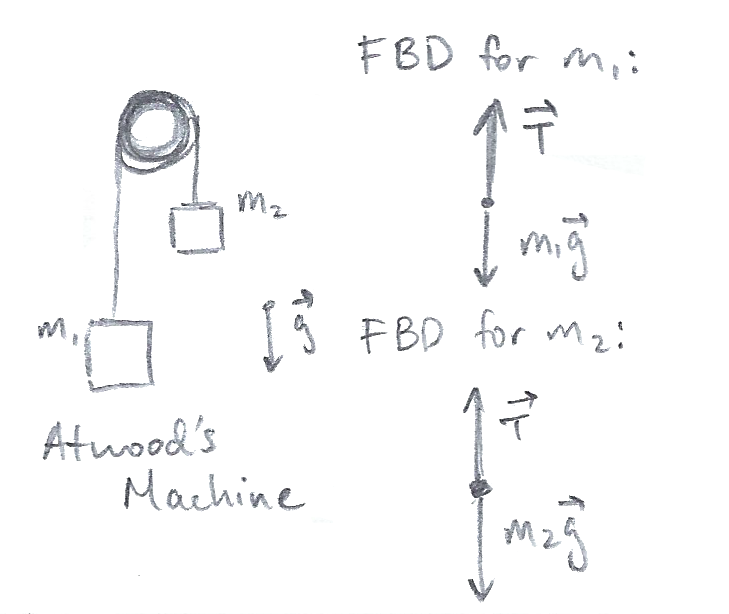
\includegraphics[width=0.5\textwidth]{images/mechintro/atwoods_machine.png}\\
\end{center}
Note that the forces only act in one direction, so we will establish a unit vector $\hat y$ upwards in order to project the components of the forces along this line. First, we do need to write Newton's Second Law for each block: 
\[
	\sum_i \vec F_i = m_1 \vec g + \vec T = m_1 \vec a
\]
\[
	\sum_i \vec F_i = m_2 \vec g + \vec T = -m_2 \vec a
\]
The only subtlety here is noting that kinematically, the blocks are attached to each other and thus have the same acceleration, except in opposite directions - when one goes up, the other must go down, and vice versa, resulting in a negative sign in front of one of the equations. \\
Now we can project along the $y$-direction:
\begin{align*}
-m_1g + T = m_1a \\
-m_2g + T = -m_2a
\end{align*}
This is a two-variable system of equations with two unknowns, so we can just solve for $T$ and $a$, which aren't particularly pretty, but are:
\[
	T = \frac{2m_1m_2}{m_1+m_2}g \quad a = \frac{m_2-m_1}{m_2+m_1}g
\]

\subsubsection{Summary and Problems}
Newton's laws of motion can be applied to situations to analyze how objects move, especially when external forces are applied to systems of objects. We also can start to figure out how objects interact with each other based on their contacts with one another. \\
There isn't much to do other than to practice the method we use to analyze dynamical situations, that being to draw correct free-body diagrams, using Newton's Second Law and projecting into components, and then solving for all unknowns using some kinematics to simplify the number of variables involved.  \\

\noindent \textbf{Problems}\\
1. (1 $\bigstar$) a) A block of mass $m$, experiencing a force of friction, slides at constant speed down a plane inclined at an angle $\theta$ with the horizontal. Show $\mu_k = \tan\theta$. b) The same block rests on a frictionless wedge inclined at an angle of $\theta$. If the wedge is accelerated with acceleration $\vec a$ so that the block remains stationary relative to the wedge, show that the magnitude of this acceleration is $a = g\tan \theta$. \\
2. (3 $\bigstar$) A stone of mass $m$ attached to a string is whirled in a horizontal circle of radius $r$. The string makes an angle of $\theta$ with the vertical, and the other end of the string is fixed directly above the center of the circle. Show the speed of the stone is $v = \sqrt{rg\tan\theta}$ and the tension in the string is $T = mg/\cos\theta $.\\
3. (2 $\bigstar$) A slide-loving pig slides down a side with angle $\theta$ in $n$ times the time it would take to slide down a frictionless slide with angle $\theta$. Show that the coefficient of kinetic friction between the pig and the first slide is $\frac{n^2-1}{n^2}\tan\theta$.\\
4. (3 $\bigstar$) A puck of mass $m$ slides in a circle of radius $r$ on a frictionless table while attached to a hanging cylinder of mass $M$ by a cord through a hole in the table. Show if that the cylinder is to remain at rest, the puck needs to be moving at a speed of $v = \sqrt{\frac{Mgr}{m}}$. \\
5. (3 $\bigstar$, $\spadesuit$) Revisit Atwood's machine, in which two containers are connected by a cord (of negligible mass) passing over a frictionless pulley (also of negligible mass). At time $t = 0$, container 1 has mass 1.30 kg and container 2 has mass 3.36 kg, but container 1 is losing mass (through a leak) at the constant rate of 0.256 kg/s. a) Show that the rate at which the acceleration magnitude of the containers changing at $t = 3.00 \, s$ is 1.11 m/s$^3$. b) Show the acceleration reaches its maximum value at $t = 5.08$ s.\\
6. (2 $\bigstar$) The floor of a railroad flatcar is loaded with loose crates having a coefficient of static friction $\mu_s$ with the floor. If the train is initially moving at a speed of $v$, show the minimum distance $\Delta x$ in which the train can be stopped at constant acceleration without causing the crates to slide over the floor is $\frac{v^2}{2g\mu_s}$.\\
7. (5 $\bigstar$) A car travels on a banked curve. The coefficient of static friction between the tires of the car and the roadway of the banked curve is $\frac{3}{4}$. The curve has radius $R$ and is banked at the incline angle so that the force of static friction is zero if the car travels with constant speed $S$. Show that the maximum speed that a car can traverse the banked curve is $SRg \sqrt{\frac{7}{4-3S^2}}$. 

\pagebreak